\subsection{Worker f�r Daten�bermittlung}\label{subsec:Worker}
Der vorliegende Abschnitt befasst sich mit dem Teil der Wissenserwerbskomponente, der als Bindeglied zwischen den Wissenserfassungsmethoden und der Wissensbasis auftritt und in Abbildung \ref{fig:wissenserwerbskomponente} als Schnittstelle f�r die Daten�bermittlung bezeichnet wird. Im Rahmen dieser Arbeit wird der Begriff \glqq{}\textit{Worker}\grqq{} verwendet, der f�r die Auspr�gung dieser Schnittstelle steht. Im Folgenden wird das Konzept hinter dem Worker abstrakt skizziert und im weiteren Verlauf mit der konkreten Implementierung verdeutlicht. Der Anwendungsbereich vom Worker wird in Abbildung \ref{fig:worker} wie folgt dargestellt:
\begin{figure}[H] 
	\centering
	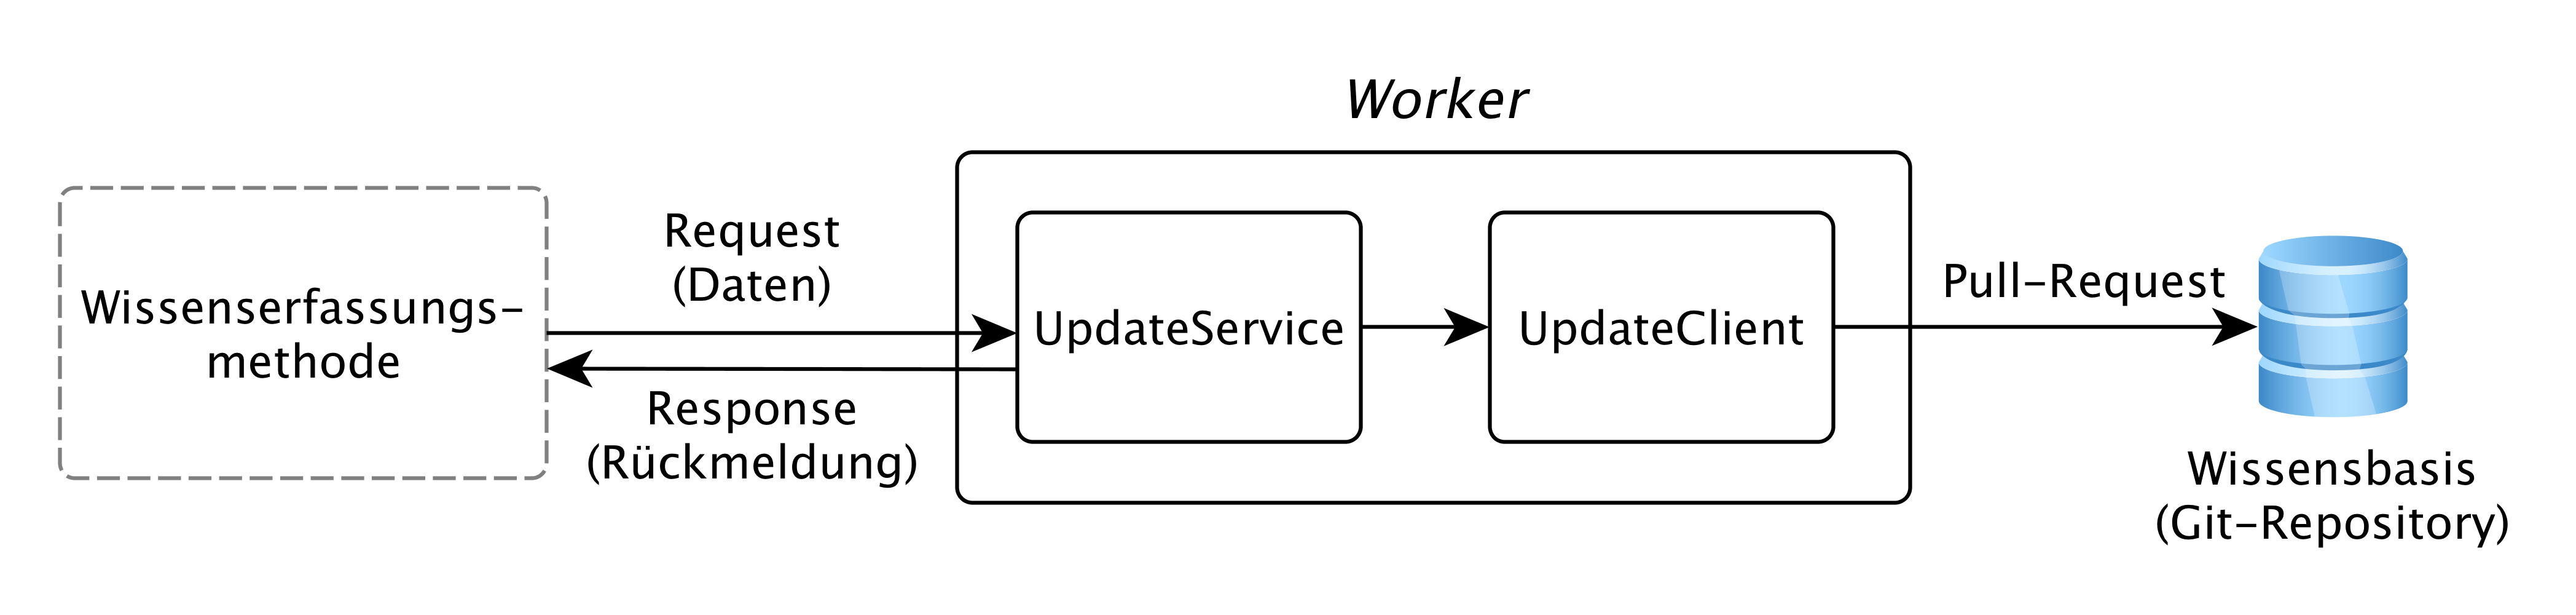
\includegraphics[width=1.0\textwidth]{images/anwendungsbereich_worker.png}
	\caption{Anwendungsbereich vom Worker}
	\label{fig:worker}
\end{figure}
Grunds�tzlich besteht der Worker aus zwei Komponenten, n�mlich \glqq{}\textit{UpdateService}\grqq{} und \glqq{}\textit{UpdateClient}\grqq{}. Die Aufgabe vom UpdateService besteht in der Bereitstellung einer Schnittstelle, die die Daten von au�en aufnimmt und die Daten�bermittlung an den UpdateClient delegiert. Auf der anderen Seite stellt der UpdateClient die Methoden zur Verf�gung, die f�r die Daten�bermittlung zust�ndig sind.\\
Generell l�sst sich der Ablauf gem�� der Abbildung \ref{fig:worker} folgenderma�en beschreiben. Als erstes werden die Daten von der Wissenserfassungsmethode an den UpdateService gesendet. Darauffolgend werden die Daten vom UpdateService verarbeitet und f�r den UpdateClient vorbereitet. Im n�chsten Schritt wird die Aufgabe der Daten�bermittlung an den UpdateClient delegiert. Der UpdateClient erstellt die Anfrage an die Wissensbasis und teilt die Antwort dem UpdateService mit. Anschlie�end verschickt der UpdateService die R�ckmeldung an die Wissenserfassungsmethode.\\ 
Im Weiteren wird die Wissenstr�gerschnittstelle aus dem Abschnitt \ref{subsec:Wissenstr�gerschnittstelle} als Wissenserfassungsmethode betrachtet. Die Wissensbasis stellt das Git-Repository von \textit{PaaSfinder} dar, das von einem Bot-Account auf Github \glqq{}geforkt\grqq{} wird\footnote{https://github.com/update-bot/paas-profiles}. In anderen Worten wird das urspr�ngliche Git-Repository von \textit{PaaSfinder} kopiert, sodass der Bot-Account einen schreibenden Zugriff auf die Wissensbasis hat.\\
Technisch gesehen erfolgt der Nachrichtenaustausch zwischen Wissenserfassungsmethode, dem Worker und der Wissensbasis auf Basis von \ac{HTTP}\footnote{https://www.w3.org/Protocols} und \ac{REST} Prinzip, das urspr�nglich aus der Dissertation von Fielding \cite{fielding2000} stammt. Das zentrale Konzept von REST basiert auf Ressourcen, die im globalen Raum mithilfe von \ac{URI}\footnote{https://tools.ietf.org/html/rfc3986} eindeutig identifiziert werden \cite[S.11,35]{tilkov2015}. Ein Vendor wird also als Ressource in JSON Format zun�chst zum Worker und darauffolgend zum Git-Repository geschickt.\\
Um die Daten von au�en empfangen zu k�nnen, implementiert der UpdateClient eine REST API, die in Form einer Route (\glqq{}/vendor\grqq{}) definiert wird. Die Route entspricht dem HTTP-Standardverb POST\footnote{https://tools.ietf.org/html/rfc7231\#section-4.3.3} und akzeptiert die Daten in JSON Format. F�r die Implementierung der Route wurde das Framework Spark\footnote{http://sparkjava.com} verwendet. Auf der Seite vom UpdateClient werden die Nachrichten als Anfragen an die Github API\footnote{https://developer.github.com/v3} mithilfe von OkHttp\footnote{https://square.github.io/okhttp}  gesendet. In Java Pseudocode l�sst sich die Route folgenderma�en beschreiben (siehe Listing \ref{service}):
\begin{lstlisting}[basicstyle=\ttfamily, label=service,
					captionpos=b, caption={\glqq{}/vendor\grqq{} Route}]
post("/vendor", "application/json", (request, response) -> {
  JsonObject data = jsonParser.parse(request.body());
  
  Branch branch = new Branch(..);       
  client.postBranch(branch);
  
  File file = new File(..);
  client.putFile(file);

  PullRequest pullRequest = new PullRequest(..);
  client.postPullRequest(pullRequest);
});
\end{lstlisting}
Als erstes werden die Daten geparsed. Danach wird ein neuer Branch erzeugt und an den UpdateClient zum Absenden weitergegeben. Sobald der Branch auf der Github-Seite erfolgreich erstellt wurde, wird die Vendor-Datei im erstellen Branch aktualisiert. Anschlie�end wird ein Pull-Request erzeugt und vom UpdateClient an das Git-Repository geschickt. Bedauerlicherweise l�sst sich der Ablauf nicht parallelisieren, da der n�chste Schnitt die erfolgreiche Ausf�hrung des vorherigen Schrittes voraussetzt. Beispielsweise setzt die Aktualisierung der Datei die Erstellung vom Branch voraus, da die Datei im erstellten Branch aktualisiert wird.\\ 
Wenn man den oben beschriebenen Ablauf auf das Beispiel mit \glqq{}Heroku\grqq{} aus dem Abschnitt \ref{subsec:Wissenstr�gerschnittstelle} �bertr�gt, ergibt sich Folgendes. Sobald der Benutzer auf \glqq{}Submit\grqq{} klickt, werden die Daten als JSON in der POST-Anfrage an den Worker gesendet, n�mlich an die Schnittstelle vom UpdateService. Das erfolgreiche Branch bzw. Pull-Request-Erstellen wird durch den Code 201 (\glqq{}Created\grqq{}) im Response der Github-API mitgeteilt (siehe Listing \ref{branch} und \ref{pullrequest}). Beim erfolgreichen Updaten der Datei wird der Statuscode 200 (\glqq{}OK\grqq{}) zur�ckgeliefert (siehe Listing \ref{file}).
\begin{lstlisting}[basicstyle=\ttfamily, breaklines=true, label=branch,
					captionpos=b, caption={Response beim erfolgreichen Branch-Erstellen}]
  protocol=http/1.1,
  code=201, 
  message=Created,
  url=https://api.github.com/repos/update-bot/paas-profiles/git/refs
\end{lstlisting}

\begin{lstlisting}[basicstyle=\ttfamily, breaklines=true, label=file,
					captionpos=b, caption={Response beim erfolgreichen File-Update}]
  protocol=http/1.1,
  code=200, 
  message=OK, 
  url=https://api.github.com/repos/update-bot/paas-profiles/contents/profiles/heroku.json
\end{lstlisting}

\begin{lstlisting}[basicstyle=\ttfamily, breaklines=true, label=pullrequest,
					captionpos=b, caption={Response beim erfolgreichen Pull-Request-Erstellen}]
  protocol=http/1.1,
  code=201,
  message=Created,
  url=https://api.github.com/repos/update-bot/paas-profiles/pulls
\end{lstlisting}
Nach der erfolgreichen Pull-Request-Erstellung kann der Update von Heroku auf Github angeschaut werden (siehe Abbildung \ref{fig:pull-requests}). In der Detailansicht werden ebenso die �nderungen explizit gezeigt. Dabei werden die gel�schten Zeilen als rot markiert und die hinzugef�gten als gr�n (siehe Abbildung \ref{fig:pull-request-detail}).
\begin{figure}[H] 
	\centering
	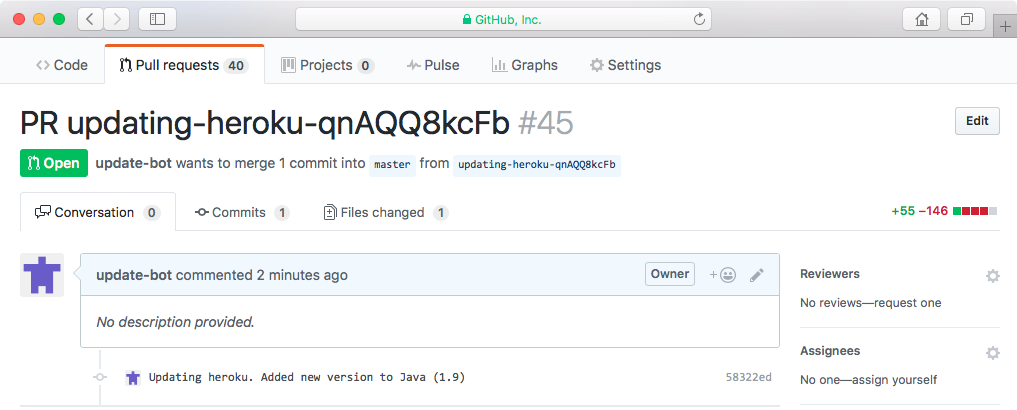
\includegraphics[width=1.0\textwidth]{images/pull-requests.png}
	\caption{Pull-Requests Ansicht auf Github}
	\label{fig:pull-requests}
\end{figure}
\begin{figure}[H] 
	\centering
	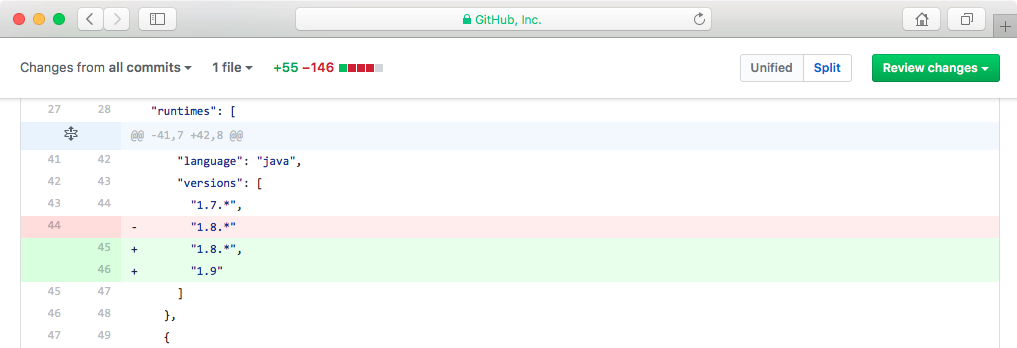
\includegraphics[width=1.0\textwidth]{images/pull-request-detail.png}
	\caption{Heroku Pull Request}
	\label{fig:pull-request-detail}
\end{figure}
Schlie�lich wird im Erfolgsfall der Statuscode 200 (\glqq{}OK\grqq{}) der Wissenserfassungsmethode mitgeteilt. In Bezug auf die Fehlerbehandlung wird jeder Schritt, der sich logisch abgrenzen l�sst (Branch erstellen, Datei aktualisieren und Pull-Request erstellen), in einem eigenen try-catch-Block bei der Route in \ref{service} ausgef�hrt, sodass der Client eine aussagekr�ftige Fehlermeldung bekommt.